 
 As seguintes ferramentas foram analisadas:
 
 
  \begin{itemize}
   \item \textit{GatherSpace \footnotemark}
      
      \begin{itemize}
       \item
	  
	  O \textit{Gatherspace} é uma ferramenta paga, porém é possível acessar a versão \textit{trial} (versão de testes) por 30 dias.
	  A ferramenta fornece uma abordagem pragmática para organizações para capturar, gerenciar, documentar, modelar
	  o negócio, teste de sistemas de requisitos;
		  
       \item
	  
	  A ferramenta apresenta uma interface com o cliente interativa e intuitiva, afim de facilitar e simplificar o processo
	  de gerenciamento de requisitos. Os relatórios são diretos e claros afim de, novamente, tornar o processo mais simples.
	  Possibilita ao usuário ficar em contato com os outros stakeholders, pois o funciona em um ambiente \textit{web} e
	  possibilita participar em múltiplos projetos. Também fornece proteção contra perda de dados como documentos apagados,
	  sobrescritos ou modificados no ambiente online;
	  
       \item
	
	  De uma maneira geral, a ferramenta apresenta uma boa abrangência no que tange ao gerenciamento de requisitos, pois
	  contém funcionalidades para tratar dos pontos importantes para uma boa realização dessa atividade, desde definição
	  de atores e requisitos de negócio até modelos de caso de uso, relatório de rastreabilidade e relatório de busca
	  de \textit{bugs}.

      \end{itemize}
      \footnotetext{Fonte: http://www.gatherspace.com/}

   \item \textit{CASE Spec \footnotemark}
      
      \begin{itemize}
       \item 
	  
	  \textit{CASE Spec} fornece soluções para os problemas de gerenciamento de ciclo de vida no desenvolvimento de software e
	  sistemas, com uma abordagem simples que evita as longas curvas de aprendizagem. Fornece recursos na área de
	  especificação de requisitos e gerenciamento, análise de requisitos, colaboração, análise de rastreabilidade,
	  especificação de \textit{design} e documentação e testes. \textit{CASE Spec} não é uma ferramenta totalmente gratuita, mas é possível
	  utilizá-la por 30 dias sem custo, sendo necessário mandar um \textit{email} para a empresa e esta responderá com o
	  \textit{link} de \textit{download} do programa;
	  
       \item
	  
	  A ferramenta fornece integração com outras ferramentas como \textit{Microsoft Word, Excel, XML}, etc, que facilitam
	  a transição de um processo puramente focado em documentos para a ferramenta. Gera automaticamente relatórios detalhados e
	  especificação de documentos. Por utilizar uma abordagem baseada na \textit{Web}, a ferramenta permite maior integração
	  de todos os \textit{stakeholders} com o fluxo de trabalho relacionado ao projeto. As especificações do sistema podem ser
	  feitas tanto em histórias de usuários quanto em casos de uso e em lista de requisitos hierárquicos.

      \end{itemize}
      \footnotetext{Fonte: http://analysttool.com/}

    \item \textit{TestTrack \footnotemark}
      \footnotetext{Fonte: http://www.seapine.com/development-activity/requirements-management}
	
      \begin{itemize}

	\item 
	
	    O \textit{TestTrack} é uma ferramenta de gerenciamento do ciclo de vida da aplicação 
	    (do inglês \textit{Application Lifecycle Management}), sendo que possui como uma de suas funcionalidades
	    o gerenciamento dos requisitos. É paga, entretanto,possui um período de testes (\textit{trial}) de 30 dias,
	    o que torna possível utilizá-la de forma gratuita;
	    
	\item
	
	    Como uma de suas características destaca-se o fato de ser versátil, possuindo cliente nas versões para \textit{Windows, Mac} e
	    \textit{Linux}, além de um cliente \textit{online} (o que possibilita sua utilização independente do sistema operacional que está
	    sendo utilizado). Possui um bom foco na interação entre a equipe, também sendo possível verificar a rastreabilidade
	    dos requisitos de forma não complexa. Um dos problemas encontrados por essa ferramenta é a necessidade de um
	    servidor para a relação cliente-servidor;
	
	\item
	
	    O ponto que se destaca é a sua flexibilidade, sendo que é possível configurá-la para projetos que usam abordagens
	    que vão desde o cascata (tradicional) até ágeis.
	    
	  \begin{figure}[!htbp]
	    \centering
	    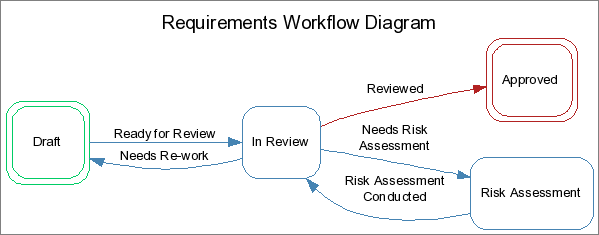
\includegraphics[scale=0.65]{editaveis/figuras/workflow_testtrack}
	    \caption[Exemplo de um diagrama de workflow de requisitos no TestTrack]
		{Diagrama de \textit{workflow} de requisitos no \textit{TestTrack}. \footnotemark}
	    \label{workflow_testtrack}
	  \end{figure}
	  \footnotetext{Disponível em: <http://www.seapine.com/images/landing/TTRMFlexibleWorkflow-599x235.png>. Acesso em 30/04/2015.}\
      
      \end{itemize}
      
  \end{itemize}
 
 